\iffalse
\documentclass[journal,12pt,twocolumn]{IEEEtran}
\def\inputGnumericTable{}
\usepackage{setspace}
\usepackage{gensymb}
\usepackage{xcolor}
\usepackage{caption}
\singlespacing
\usepackage{siunitx}
\usepackage[cmex10]{amsmath}
\usepackage{mathtools}
\usepackage{hyperref}
\usepackage{amsthm}
\usepackage{mathrsfs}
\usepackage{txfonts}
\usepackage{stfloats}
\usepackage{cite}
\usepackage{cases}
\usepackage{subfig}
\usepackage{longtable}
\usepackage{multirow}
\usepackage{enumitem}
\usepackage{mathtools}
\usepackage{listings}
\usepackage{tikz}
\usetikzlibrary{shapes,arrows,positioning}
\usepackage{circuitikz}
       \usepackage[latin1]{inputenc}
       \usepackage{fullpage}
       \usepackage{color}
       \usepackage{array}
       \usepackage{longtable}
       \usepackage{calc}
       \usepackage{multirow}
       \usepackage{hhline}
       \usepackage{ifthen}
	   \usepackage{setspace}
\let\vec\mathbf
\DeclareMathOperator*{\Res}{Res}
\renewcommand\thesection{\arabic{section}}
\renewcommand\thesubsection{\thesection.\arabic{subsection}}
\renewcommand\thesubsubsection{\thesubsection.\arabic{subsubsection}}

\renewcommand\thesectiondis{\arabic{section}}
\renewcommand\thesubsectiondis{\thesectiondis.\arabic{subsection}}
\renewcommand\thesubsubsectiondis{\thesubsectiondis.\arabic{subsubsection}}
\hyphenation{op-tical net-works semi-conduc-tor}

\lstset{
language=Python,
frame=single, 
breaklines=true,
columns=fullflexible
}
\begin{document}
\theoremstyle{definition}
\newtheorem{theorem}{Theorem}[section]
\newtheorem{problem}{Problem}
\newtheorem{proposition}{Proposition}[section]
\newtheorem{lemma}{Lemma}[section]
\newtheorem{corollary}[theorem]{Corollary}
\newtheorem{example}{Example}[section]
\newtheorem{definition}{Definition}[section]
\newcommand{\BEQA}{\begin{eqnarray}}
        \newcommand{\EEQA}{\end{eqnarray}}
\newcommand{\define}{\stackrel{\triangle}{=}}
\newcommand{\myvec}[1]{\ensuremath{\begin{pmatrix}#1\end{pmatrix}}}
\newcommand{\mydet}[1]{\ensuremath{\begin{vmatrix}#1\end{vmatrix}}}

\bibliographystyle{IEEEtran}
\providecommand{\nCr}[2]{\,^{#1}C_{#2}} % nCr
\providecommand{\nPr}[2]{\,^{#1}P_{#2}} % nPr
\providecommand{\mbf}{\mathbf}
\providecommand{\pr}[1]{\ensuremath{\Pr\left(#1\right)}}
\providecommand{\qfunc}[1]{\ensuremath{Q\left(#1\right)}}
\providecommand{\sbrak}[1]{\ensuremath{{}\left[#1\right]}}
\providecommand{\lsbrak}[1]{\ensuremath{{}\left[#1\right.}}
\providecommand{\rsbrak}[1]{\ensuremath{{}\left.#1\right]}}
\providecommand{\brak}[1]{\ensuremath{\left(#1\right)}}
\providecommand{\lbrak}[1]{\ensuremath{\left(#1\right.}}
\providecommand{\rbrak}[1]{\ensuremath{\left.#1\right)}}
\providecommand{\cbrak}[1]{\ensuremath{\left\{#1\right\}}}
\providecommand{\lcbrak}[1]{\ensuremath{\left\{#1\right.}}
\providecommand{\rcbrak}[1]{\ensuremath{\left.#1\right\}}}
\theoremstyle{remark}
\newtheorem{rem}{Remark}
\newcommand{\sgn}{\mathop{\mathrm{sgn}}}
\newcommand{\rect}{\mathop{\mathrm{rect}}}
\newcommand{\sinc}{\mathop{\mathrm{sinc}}}
\providecommand{\abs}[1]{\left\vert#1\right\vert}
\providecommand{\res}[1]{\Res\displaylimits_{#1}}
\providecommand{\norm}[1]{\lVert#1\rVert}
\providecommand{\mtx}[1]{\mathbf{#1}}
\providecommand{\mean}[1]{E\left[ #1 \right]}
\providecommand{\fourier}{\overset{\mathcal{F}}{ \rightleftharpoons}}
\providecommand{\ztrans}{\overset{\mathcal{Z}}{ \rightleftharpoons}}
\providecommand{\system}[1]{\overset{\mathcal{#1}}{ \longleftrightarrow}}
\newcommand{\solution}{\noindent \textbf{Solution: }}
\providecommand{\dec}[2]{\ensuremath{\overset{#1}{\underset{#2}{\gtrless}}}}
\let\StandardTheFigure\thefigure
\def\putbox#1#2#3{\makebox[0in][l]{\makebox[#1][l]{}\raisebox{\baselineskip}[0in][0in]{\raisebox{#2}[0in][0in]{#3}}}}
\def\rightbox#1{\makebox[0in][r]{#1}}
\def\centbox#1{\makebox[0in]{#1}}
\def\topbox#1{\raisebox{-\baselineskip}[0in][0in]{#1}}
\def\midbox#1{\raisebox{-0.5\baselineskip}[0in][0in]{#1}}

\vspace{3cm}
\title{\LaTeX\ 9.10.6.7}
\author{Lokesh Surana}
\maketitle
\section*{Class 9, Chapter, 10, Exercse 6.7}


\solution
\fi
Consider a unit circle with center at origin.
Let $AC$ and $BD$ be the diameters of the circle.
The points on circle that we consider are available in Table \eqref{tab:chapters/9/10/6/7/points}.
%
\begin{table}[ht!]
\begin{tabular}{|c|c|p{5cm}|}
\hline
\textbf{Symbol} & \textbf{Value} & \textbf{Description} \\
\hline
$\theta$ & $30\degree$ & $\angle{BAP} = \angle{BAQ}$ \\
\hline
$a$ & $9$ & $AB$ \\
\hline
$c$ & $8$ & $AQ$ \\
\hline
$\vec{e}_1$ & $\myvec{1\\0}$ & Basis vector \\
\hline
\end{tabular}

\caption{}
\label{tab:chapters/9/10/6/7/points}
\end{table}
%
\begin{enumerate}
    \item $AC$ and $BD$ are diameters of the circle. Let's check if they bisect each other,
    \begin{align}
        \vec{A} + \vec{C} &= \myvec{1 \\ 0} + \myvec{-1 \\ 0}\\
        \label{eq:chapters/9/10/6/7/1} &= \myvec{0 \\ 0} \\
        \vec{B} + \vec{D} &= \myvec{1 \\ 0} + \myvec{-1 \\ 0}\\
        \label{eq:chapters/9/10/6/7/2} &= \myvec{0 \\ 0}
    \end{align}
    From equation \eqref{eq:chapters/9/10/6/7/1} and \eqref{eq:chapters/9/10/6/7/2} $AC$ and $BD$ bisect each other.
    Hence, we can say that if two chords bisect each other then they are diameters.
%
    \item Let's check if $ABCD$ is a rectangle.
    The sides of a rectangle are parallel to each other. Let's check if $AB$ and $BC$ are parallel to each other.
    \begin{align}
        \vec{A} - \vec{B} &= \myvec{1 \\ 0} - \myvec{0 \\ 1}\\
        \label{eq:chapters/9/10/6/7/4} &= \myvec{1 \\ -1} \\
        \vec{D} - \vec{C} &= \myvec{0\\ -1} - \myvec{-1 \\ 0}\\
        \label{eq:chapters/9/10/6/7/5} &= \myvec{1 \\ -1} 
    \end{align}
    From equation \eqref{eq:chapters/9/10/6/7/4} and \eqref{eq:chapters/9/10/6/7/5}, $AB$ and $DC$ are parallel to each other.
    $\implies ABCD$ is a parallelogram.

    Now let's check if its a rectangle.
    Let's check the angle between adjacent sides of this quadrilateral, i.e. $AB$ and $BC$.
    \begin{align}
        \label{eq:chapters/9/10/6/7/6} \brak{\vec{A} - \vec{B}}^\top \brak{\vec{B} - \vec{C}} &=  \myvec{1 & -1} \myvec{1 \\ 1} \\
        &= 0
    \end{align}
    From equation \eqref{eq:chapters/9/10/6/7/6}, we can say that the angle between $AB$ and $BC$ is $90\degree$.
    Hence, the quadrilateral $ABCD$ is a rectangle.
\end{enumerate}

\begin{figure}[!htb]
    \centering
    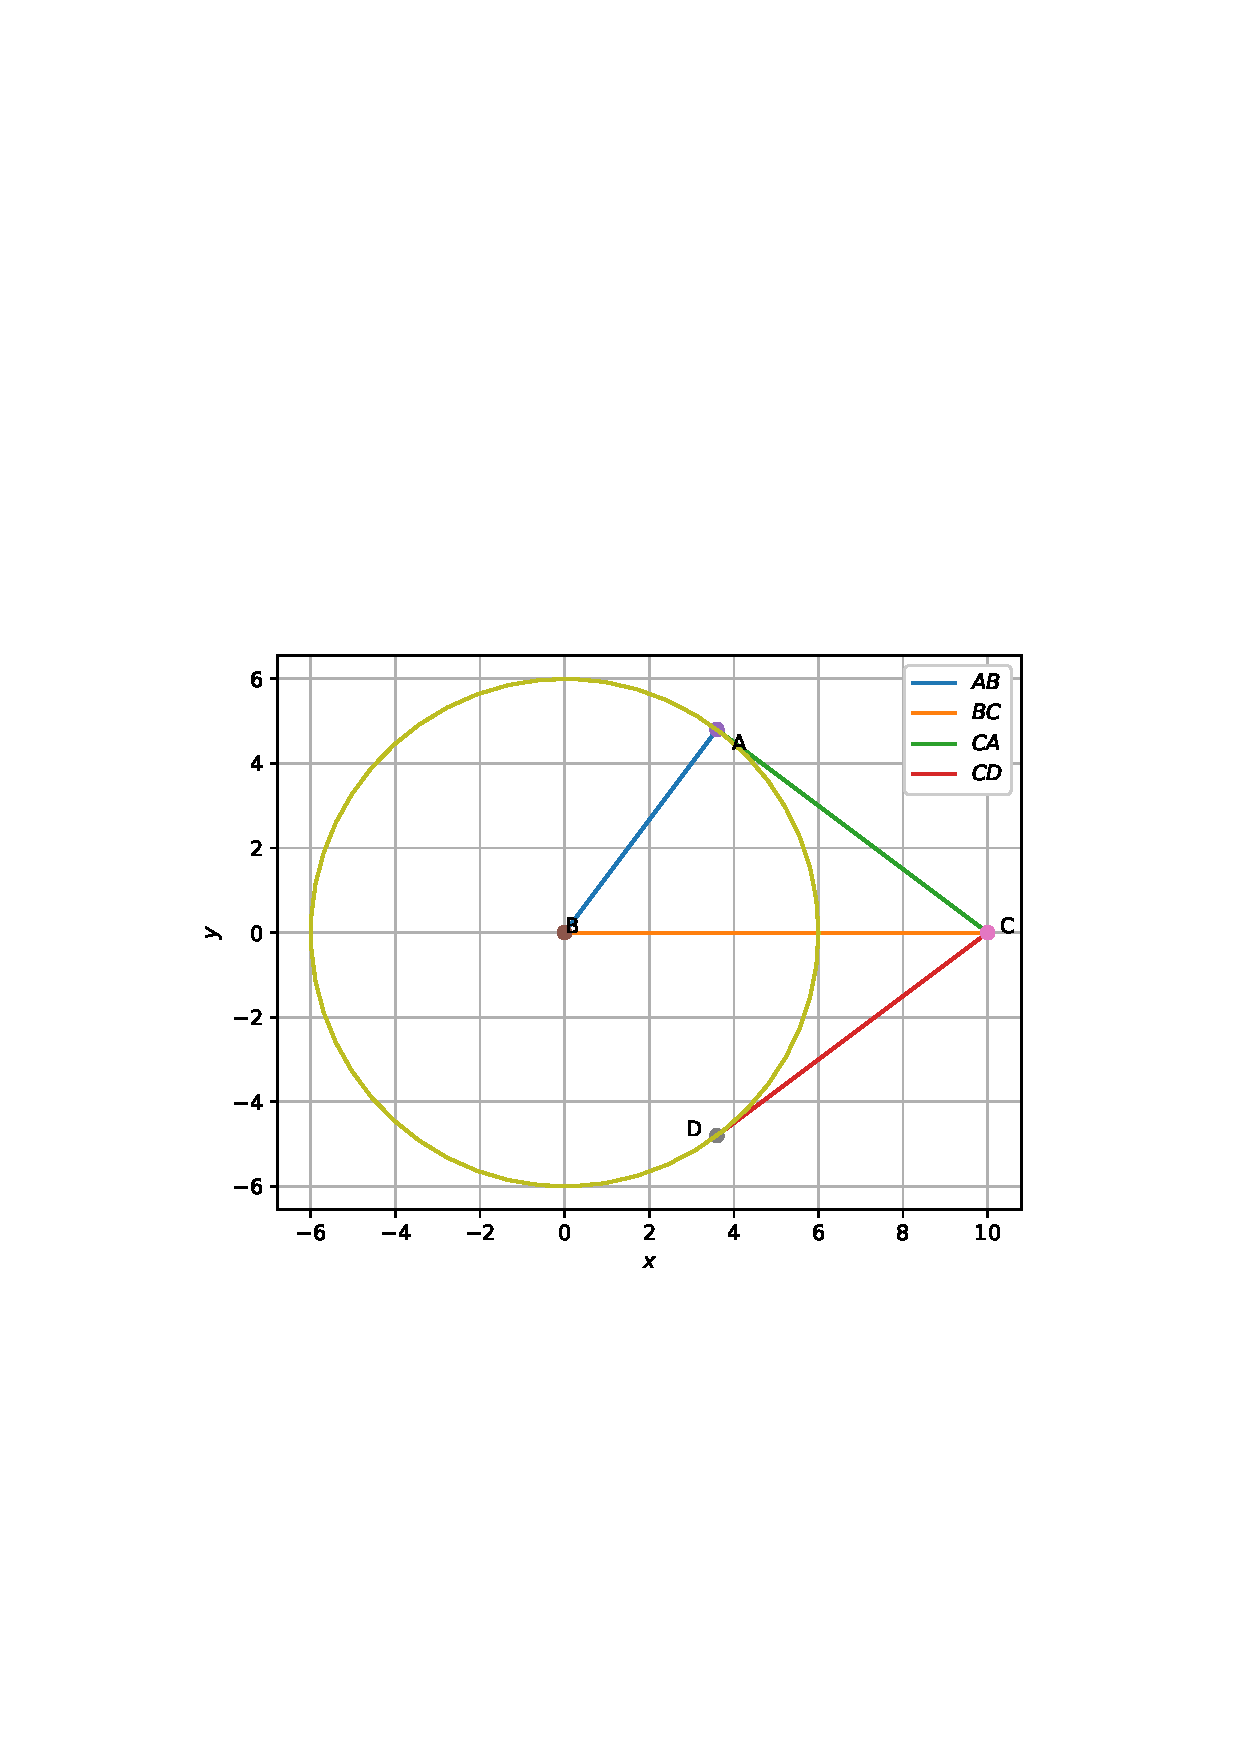
\includegraphics[width=\columnwidth]{chapters/9/10/6/7/figs/circle.png}
    \caption{circle}
    \label{fig:chapters/9/10/6/7/circle}
\end{figure}

